% Created by tikzDevice version 0.6.2-92-0ad2792 on 2014-03-27 04:41:27
% !TEX encoding = UTF-8 Unicode
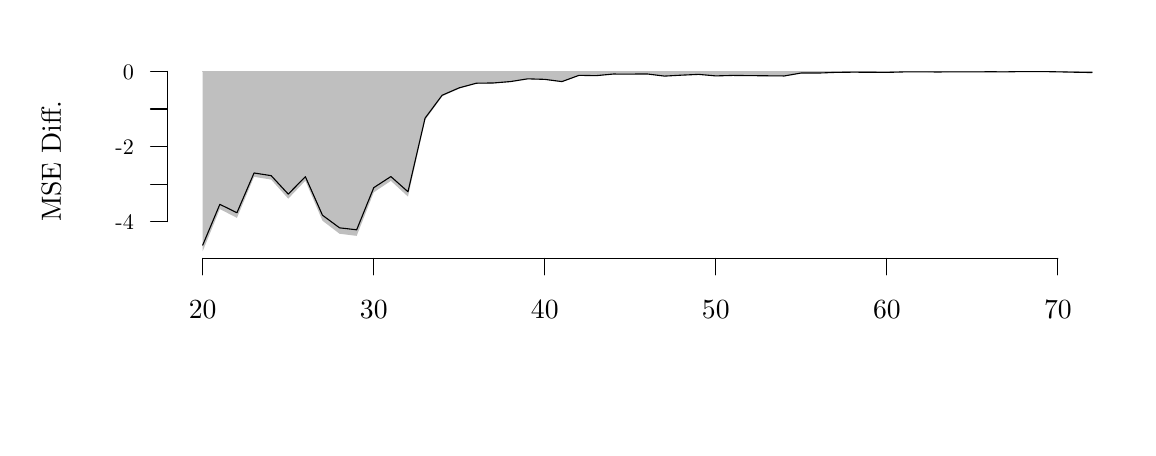
\begin{tikzpicture}[x=1pt,y=1pt]
\definecolor[named]{fillColor}{rgb}{1.00,1.00,1.00}
\path[use as bounding box,fill=fillColor,fill opacity=0.00] (0,0) rectangle (397.48,144.54);
\begin{scope}
\path[clip] ( 50.40, 61.20) rectangle (397.48,131.34);
\definecolor[named]{drawColor}{rgb}{1.00,1.00,1.00}

\path[draw=drawColor,line width= 0.3pt,line join=round,line cap=round] ( 63.25, 63.80) --
	( 69.44, 79.00) --
	( 75.62, 75.81) --
	( 81.80, 90.65) --
	( 87.98, 89.65) --
	( 94.16, 82.75) --
	(100.34, 89.24) --
	(106.52, 74.79) --
	(112.70, 70.07) --
	(118.88, 69.31) --
	(125.06, 85.04) --
	(131.24, 89.19) --
	(137.42, 83.50) --
	(143.60,111.13) --
	(149.78,119.75) --
	(155.96,122.55) --
	(162.14,124.28) --
	(168.32,124.38) --
	(174.50,124.90) --
	(180.68,125.93) --
	(186.86,125.73) --
	(193.04,124.88) --
	(199.22,127.25) --
	(205.40,127.14) --
	(211.58,127.74) --
	(217.76,127.73) --
	(223.94,127.76) --
	(230.12,126.96) --
	(236.30,127.32) --
	(242.48,127.60) --
	(248.66,127.03) --
	(254.84,127.21) --
	(261.02,127.14) --
	(267.20,127.07) --
	(273.38,127.01) --
	(279.57,128.12) --
	(285.75,128.10) --
	(291.93,128.34) --
	(298.11,128.42) --
	(304.29,128.39) --
	(310.47,128.33) --
	(316.65,128.52) --
	(322.83,128.54) --
	(329.01,128.49) --
	(335.19,128.54) --
	(341.37,128.53) --
	(347.55,128.56) --
	(353.73,128.53) --
	(359.91,128.64) --
	(366.09,128.64) --
	(372.27,128.53) --
	(378.45,128.38) --
	(384.63,128.25);

\path[draw=drawColor,line width= 0.3pt,line join=round,line cap=round] ( 63.25, 65.95) --
	( 69.44, 80.70) --
	( 75.62, 77.67) --
	( 81.80, 92.03) --
	( 87.98, 91.07) --
	( 94.16, 84.40) --
	(100.34, 90.69) --
	(106.52, 76.77) --
	(112.70, 72.21) --
	(118.88, 71.50) --
	(125.06, 86.73) --
	(131.24, 90.74) --
	(137.42, 85.25) --
	(143.60,111.86) --
	(149.78,120.13) --
	(155.96,122.81) --
	(162.14,124.47) --
	(168.32,124.56) --
	(174.50,125.07) --
	(180.68,126.05) --
	(186.86,125.86) --
	(193.04,125.05) --
	(199.22,127.31) --
	(205.40,127.20) --
	(211.58,127.78) --
	(217.76,127.77) --
	(223.94,127.80) --
	(230.12,127.04) --
	(236.30,127.38) --
	(242.48,127.66) --
	(248.66,127.11) --
	(254.84,127.28) --
	(261.02,127.21) --
	(267.20,127.15) --
	(273.38,127.09) --
	(279.57,128.17) --
	(285.75,128.14) --
	(291.93,128.38) --
	(298.11,128.46) --
	(304.29,128.43) --
	(310.47,128.38) --
	(316.65,128.55) --
	(322.83,128.57) --
	(329.01,128.53) --
	(335.19,128.58) --
	(341.37,128.57) --
	(347.55,128.60) --
	(353.73,128.58) --
	(359.91,128.68) --
	(366.09,128.68) --
	(372.27,128.58) --
	(378.45,128.44) --
	(384.63,128.32);

\path[draw=drawColor,line width= 0.3pt,line join=round,line cap=round] ( 63.25,128.74) --
	( 69.44,128.74) --
	( 75.62,128.74) --
	( 81.80,128.74) --
	( 87.98,128.74) --
	( 94.16,128.74) --
	(100.34,128.74) --
	(106.52,128.74) --
	(112.70,128.74) --
	(118.88,128.74) --
	(125.06,128.74) --
	(131.24,128.74) --
	(137.42,128.74) --
	(143.60,128.74) --
	(149.78,128.74) --
	(155.96,128.74) --
	(162.14,128.74) --
	(168.32,128.74) --
	(174.50,128.74) --
	(180.68,128.74) --
	(186.86,128.74) --
	(193.04,128.74) --
	(199.22,128.74) --
	(205.40,128.74) --
	(211.58,128.74) --
	(217.76,128.74) --
	(223.94,128.74) --
	(230.12,128.74) --
	(236.30,128.74) --
	(242.48,128.74) --
	(248.66,128.74) --
	(254.84,128.74) --
	(261.02,128.74) --
	(267.20,128.74) --
	(273.38,128.74) --
	(279.57,128.74) --
	(285.75,128.74) --
	(291.93,128.74) --
	(298.11,128.74) --
	(304.29,128.74) --
	(310.47,128.74) --
	(316.65,128.74) --
	(322.83,128.74) --
	(329.01,128.74) --
	(335.19,128.74) --
	(341.37,128.74) --
	(347.55,128.74) --
	(353.73,128.74) --
	(359.91,128.74) --
	(366.09,128.74) --
	(372.27,128.74) --
	(378.45,128.74) --
	(384.63,128.74);
\end{scope}
\begin{scope}
\path[clip] (  0.00,  0.00) rectangle (397.48,144.54);
\definecolor[named]{drawColor}{rgb}{0.00,0.00,0.00}

\node[text=drawColor,rotate= 90.00,anchor=base,inner sep=0pt, outer sep=0pt, scale=  1.00] at ( 12.00, 96.27) {MSE Diff.};
\end{scope}
\begin{scope}
\path[clip] (  0.00,  0.00) rectangle (397.48,144.54);
\definecolor[named]{drawColor}{rgb}{0.00,0.00,0.00}

\path[draw=drawColor,line width= 0.4pt,line join=round,line cap=round] ( 63.25, 61.20) -- (372.27, 61.20);

\path[draw=drawColor,line width= 0.4pt,line join=round,line cap=round] ( 63.25, 61.20) -- ( 63.25, 55.20);

\path[draw=drawColor,line width= 0.4pt,line join=round,line cap=round] (125.06, 61.20) -- (125.06, 55.20);

\path[draw=drawColor,line width= 0.4pt,line join=round,line cap=round] (186.86, 61.20) -- (186.86, 55.20);

\path[draw=drawColor,line width= 0.4pt,line join=round,line cap=round] (248.66, 61.20) -- (248.66, 55.20);

\path[draw=drawColor,line width= 0.4pt,line join=round,line cap=round] (310.47, 61.20) -- (310.47, 55.20);

\path[draw=drawColor,line width= 0.4pt,line join=round,line cap=round] (372.27, 61.20) -- (372.27, 55.20);

\node[text=drawColor,anchor=base,inner sep=0pt, outer sep=0pt, scale=  1.00] at ( 63.25, 39.60) {20};

\node[text=drawColor,anchor=base,inner sep=0pt, outer sep=0pt, scale=  1.00] at (125.06, 39.60) {30};

\node[text=drawColor,anchor=base,inner sep=0pt, outer sep=0pt, scale=  1.00] at (186.86, 39.60) {40};

\node[text=drawColor,anchor=base,inner sep=0pt, outer sep=0pt, scale=  1.00] at (248.66, 39.60) {50};

\node[text=drawColor,anchor=base,inner sep=0pt, outer sep=0pt, scale=  1.00] at (310.47, 39.60) {60};

\node[text=drawColor,anchor=base,inner sep=0pt, outer sep=0pt, scale=  1.00] at (372.27, 39.60) {70};
\end{scope}
\begin{scope}
\path[clip] ( 50.40, 61.20) rectangle (397.48,131.34);
\definecolor[named]{fillColor}{rgb}{0.75,0.75,0.75}

\path[fill=fillColor] ( 63.25,128.74) --
	( 63.25, 63.80) --
	( 69.44, 79.00) --
	( 75.62, 75.81) --
	( 81.80, 90.65) --
	( 87.98, 89.65) --
	( 94.16, 82.75) --
	(100.34, 89.24) --
	(106.52, 74.79) --
	(112.70, 70.07) --
	(118.88, 69.31) --
	(125.06, 85.04) --
	(131.24, 89.19) --
	(137.42, 83.50) --
	(143.60,111.13) --
	(149.78,119.75) --
	(155.96,122.55) --
	(162.14,124.28) --
	(168.32,124.38) --
	(174.50,124.90) --
	(180.68,125.93) --
	(186.86,125.73) --
	(193.04,124.88) --
	(199.22,127.25) --
	(205.40,127.14) --
	(211.58,127.74) --
	(217.76,127.73) --
	(223.94,127.76) --
	(230.12,126.96) --
	(236.30,127.32) --
	(242.48,127.60) --
	(248.66,127.03) --
	(254.84,127.21) --
	(261.02,127.14) --
	(267.20,127.07) --
	(273.38,127.01) --
	(279.57,128.12) --
	(285.75,128.10) --
	(291.93,128.34) --
	(298.11,128.42) --
	(304.29,128.39) --
	(310.47,128.33) --
	(316.65,128.52) --
	(322.83,128.54) --
	(329.01,128.49) --
	(335.19,128.54) --
	(341.37,128.53) --
	(347.55,128.56) --
	(353.73,128.53) --
	(359.91,128.64) --
	(366.09,128.64) --
	(372.27,128.53) --
	(378.45,128.38) --
	(384.63,128.25) --
	(384.63,128.74) --
	cycle;
\definecolor[named]{drawColor}{rgb}{0.75,0.75,0.75}

\path[draw=drawColor,line width= 0.4pt,line join=round,line cap=round] ( 63.25,128.74) --
	(384.63,128.74);
\definecolor[named]{drawColor}{rgb}{0.00,0.00,0.00}

\path[draw=drawColor,line width= 0.4pt,line join=round,line cap=round] ( 63.25, 65.95) --
	( 69.44, 80.70) --
	( 75.62, 77.67) --
	( 81.80, 92.03) --
	( 87.98, 91.07) --
	( 94.16, 84.40) --
	(100.34, 90.69) --
	(106.52, 76.77) --
	(112.70, 72.21) --
	(118.88, 71.50) --
	(125.06, 86.73) --
	(131.24, 90.74) --
	(137.42, 85.25) --
	(143.60,111.86) --
	(149.78,120.13) --
	(155.96,122.81) --
	(162.14,124.47) --
	(168.32,124.56) --
	(174.50,125.07) --
	(180.68,126.05) --
	(186.86,125.86) --
	(193.04,125.05) --
	(199.22,127.31) --
	(205.40,127.20) --
	(211.58,127.78) --
	(217.76,127.77) --
	(223.94,127.80) --
	(230.12,127.04) --
	(236.30,127.38) --
	(242.48,127.66) --
	(248.66,127.11) --
	(254.84,127.28) --
	(261.02,127.21) --
	(267.20,127.15) --
	(273.38,127.09) --
	(279.57,128.17) --
	(285.75,128.14) --
	(291.93,128.38) --
	(298.11,128.46) --
	(304.29,128.43) --
	(310.47,128.38) --
	(316.65,128.55) --
	(322.83,128.57) --
	(329.01,128.53) --
	(335.19,128.58) --
	(341.37,128.57) --
	(347.55,128.60) --
	(353.73,128.58) --
	(359.91,128.68) --
	(366.09,128.68) --
	(372.27,128.58) --
	(378.45,128.44) --
	(384.63,128.32);
\end{scope}
\begin{scope}
\path[clip] (  0.00,  0.00) rectangle (397.48,144.54);
\definecolor[named]{drawColor}{rgb}{0.00,0.00,0.00}

\path[draw=drawColor,line width= 0.4pt,line join=round,line cap=round] ( 50.40, 74.43) -- ( 50.40,128.74);

\path[draw=drawColor,line width= 0.4pt,line join=round,line cap=round] ( 50.40, 74.43) -- ( 44.40, 74.43);

\path[draw=drawColor,line width= 0.4pt,line join=round,line cap=round] ( 50.40, 88.01) -- ( 44.40, 88.01);

\path[draw=drawColor,line width= 0.4pt,line join=round,line cap=round] ( 50.40,101.59) -- ( 44.40,101.59);

\path[draw=drawColor,line width= 0.4pt,line join=round,line cap=round] ( 50.40,115.16) -- ( 44.40,115.16);

\path[draw=drawColor,line width= 0.4pt,line join=round,line cap=round] ( 50.40,128.74) -- ( 44.40,128.74);

\node[text=drawColor,anchor=base east,inner sep=0pt, outer sep=0pt, scale=  0.80] at ( 38.40, 71.68) {-4};

\node[text=drawColor,anchor=base east,inner sep=0pt, outer sep=0pt, scale=  0.80] at ( 38.40, 98.83) {-2};

\node[text=drawColor,anchor=base east,inner sep=0pt, outer sep=0pt, scale=  0.80] at ( 38.40,125.99) {0};
\end{scope}
\end{tikzpicture}
